\begin{figure}
    \centering

    \tikzset {_efbsk5dva/.code = {\pgfsetadditionalshadetransform{ \pgftransformshift{\pgfpoint{89.1 bp } { -128.7 bp }  }  \pgftransformscale{1.32 }  }}}
    \pgfdeclareradialshading{_ah1a1en88}{\pgfpoint{-72bp}{104bp}}{rgb(0bp)=(1,1,1);
    rgb(0bp)=(1,1,1);
    rgb(25bp)=(0.48,0.15,0.15);
    rgb(400bp)=(0.48,0.15,0.15)}
    \tikzset{every picture/.style={line width=0.75pt}} %set default line width to 0.75pt

    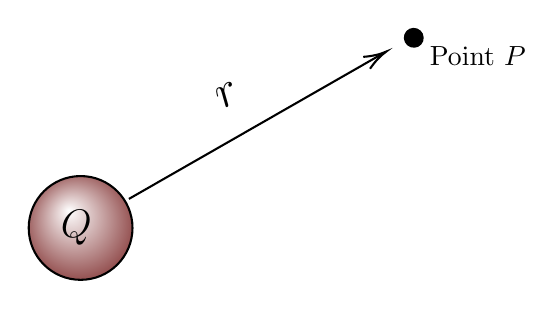
\begin{tikzpicture}[x=0.75pt,y=0.75pt,yscale=-1,xscale=1]
%uncomment if require: \path (0,300); %set diagram left start at 0, and has height of 300

%Shape: Circle [id:dp9020583883547655]
        \path  [shading=_ah1a1en88,_efbsk5dva] (93,220) .. controls (93,206.19) and (104.19,195) .. (118,195) .. controls (131.81,195) and (143,206.19) .. (143,220) .. controls (143,233.81) and (131.81,245) .. (118,245) .. controls (104.19,245) and (93,233.81) .. (93,220) -- cycle ; % for fading
        \draw   (93,220) .. controls (93,206.19) and (104.19,195) .. (118,195) .. controls (131.81,195) and (143,206.19) .. (143,220) .. controls (143,233.81) and (131.81,245) .. (118,245) .. controls (104.19,245) and (93,233.81) .. (93,220) -- cycle ; % for border

%Straight Lines [id:da31486330865489753]
        \draw    (141.3,206) -- (263.56,135.99) ;
        \draw [shift={(265.3,135)}, rotate = 510.21] [color={rgb, 255:red, 0; green, 0; blue, 0 }  ][line width=0.75]    (10.93,-3.29) .. controls (6.95,-1.4) and (3.31,-0.3) .. (0,0) .. controls (3.31,0.3) and (6.95,1.4) .. (10.93,3.29)   ;
%Shape: Circle [id:dp26251024335558126]
        \draw  [fill={rgb, 255:red, 0; green, 0; blue, 0 }  ,fill opacity=1 ] (274.24,128.58) .. controls (274.11,126.22) and (275.92,124.22) .. (278.28,124.11) .. controls (280.64,124.01) and (282.67,125.84) .. (282.8,128.2) .. controls (282.93,130.56) and (281.13,132.56) .. (278.76,132.67) .. controls (276.4,132.77) and (274.38,130.94) .. (274.24,128.58) -- cycle ;

% Text Node
        \draw (107,210) node [anchor=north west][inner sep=0.75pt]  [font=\Large] [align=left] {$\displaystyle Q$};
% Text Node
        \draw (284.8,131.2) node [anchor=north west][inner sep=0.75pt]   [align=left] {Point $P$};
% Text Node
        \draw (180,154) node [anchor=north west][inner sep=0.75pt]  [font=\LARGE,rotate=-330.07] [align=left] {$\displaystyle r$};


    \end{tikzpicture}
    \caption{A point $P$ at a distance $r$ from a charge $Q$.}
    \label{fig:potential}
\end{figure}